\documentclass[tikz,border=7pt]{standalone}
\usepackage[T1]{fontenc}
\usepackage{lmodern}
\usetikzlibrary{arrows.meta,positioning,shapes.geometric,fit,backgrounds,calc}
\begin{document}
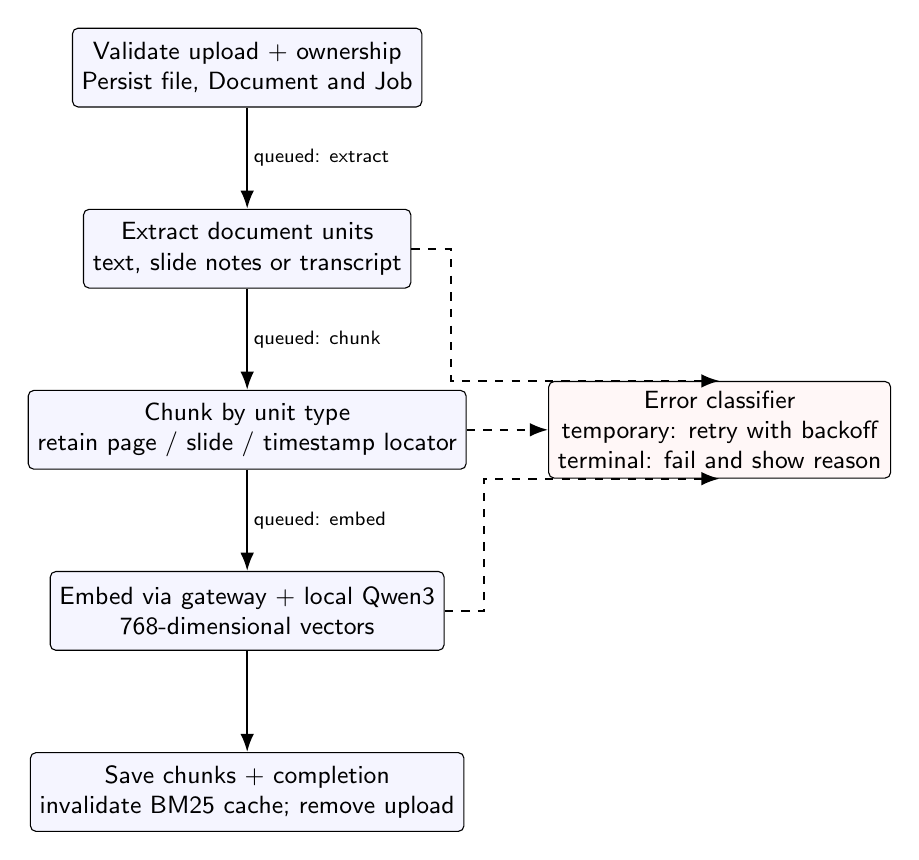
\begin{tikzpicture}[font=\sffamily\small,>=Latex,
box/.style={draw,rounded corners=2pt,align=center,minimum width=3cm,minimum height=1cm,fill=blue!4},
entity/.style={draw,rectangle,align=center,minimum width=2.6cm,minimum height=.75cm,fill=blue!4},
rel/.style={draw,diamond,aspect=2,inner sep=2pt,align=center,font=\sffamily\footnotesize,fill=yellow!8},
attr/.style={draw,ellipse,inner sep=3pt,font=\sffamily\footnotesize},
uc/.style={draw,ellipse,align=center,minimum width=4cm,minimum height=.9cm},
flow/.style={->,thick},lab/.style={font=\sffamily\scriptsize,fill=white,inner sep=2pt}]

\node[box] (upload) at (0,7) {Validate upload + ownership\\Persist file, Document and Job};
\node[box] (extract) at (0,4.7) {Extract document units\\text, slide notes or transcript};
\node[box] (chunk) at (0,2.4) {Chunk by unit type\\retain page / slide / timestamp locator};
\node[box] (embed) at (0,.1) {Embed via gateway + local Qwen3\\768-dimensional vectors};
\node[box] (save) at (0,-2.2) {Save chunks + completion\\invalidate BM25 cache; remove upload};
\node[box,fill=red!3] (error) at (6,2.4) {Error classifier\\temporary: retry with backoff\\terminal: fail and show reason};
\draw[flow] (upload) -- node[lab,right]{queued: extract} (extract);
\draw[flow] (extract) -- node[lab,right]{queued: chunk} (chunk);
\draw[flow] (chunk) -- node[lab,right]{queued: embed} (embed);
\draw[flow] (embed) -- (save);
\draw[flow,dashed] (extract.east) -- ++(.5,0) |- (error.north);
\draw[flow,dashed] (chunk.east) -- (error.west);
\draw[flow,dashed] (embed.east) -- ++(.5,0) |- (error.south);
\end{tikzpicture}
\end{document}
